\documentclass[a4paper]{report}

\usepackage{natbib}
\bibpunct{[}{]}{,}{a}{}{;}
\usepackage{fancyheadings}
\usepackage{iamdip}
\usepackage[pdftex]{graphicx}
\usepackage{subfig}
\usepackage{amsmath}
\usepackage{amsthm}
\usepackage{amssymb}
\usepackage{amsfonts}
\usepackage{url}
\usepackage{hyperref}
\usepackage{listings}

\usepackage{pdfpages}


\headrulewidth 0.5pt \addtolength{\headheight}{5pt}

\lhead[\fancyplain{}{\rm\thepage}]{\fancyplain{}{\rightmark}}
\rhead[\fancyplain{}{\leftmark}]{\fancyplain{}{\rm\thepage}}
\cfoot{}

\graphicspath{{../Figures/}}

\begin{document}

\pagestyle{fancyplain} \thispagestyle{empty}

\title{Learning Structure from Motion}
\author{Adrian W\"alchli}
\betreuer{Prof. Dr. Paolo Favaro}
\ort{Bern}
\datum{2017}

\pagenumbering{roman} \setcounter{page}{1}
\maketitle

\newpage
\thispagestyle{empty}
\vspace{8cm}
\noindent
{\centerline {\bf \large Abstract}}
\vspace{1cm}


\noindent

%abstract



\pagenumbering{roman} \setcounter{page}{1}
\tableofcontents

\newpage{\pagestyle{empty} \cleardoublepage}

% Hauptdokument
\pagenumbering{arabic} \setcounter{page}{1}
\pagestyle{fancy}

\chapter{Prior Work}

	\todo{Add text that introduces the chapter}
	
		
	\section{04/2017 - SfM-Net}

		\cite{SFMNET} implement a deep learning approach to structure from motion. 
		Their architecture consists of two subnetworks:
		\begin{itemize}
			\item \textbf{Structure }
				\\
				Learns per-frame depth.
				The input is a single frame. 
				The output of the CNN is a cloud of 3D points, one for each pixel value in the input image.
			\item \textbf{Motion}
				\\
				The input is a pair of frames.
				The CNN computes a set of $K$ segmentation masks for moving objects. 
				Using these masks, each pixel is assigned to an object specific transformation given by a rotation and a translation.
				In addition, camera rotation and translation are computed using the features of the inner layers.
		\end{itemize}
		Given a pair of images, the forward operation of the network works as follows:
		\begin{enumerate}
			\item The structure network computes the point cloud for the first frame.
			\item The motion network computes the object transformations as well as the camera transformation using both frames.
			\item The point cloud is transformed using the learned object transformations and masks.
			\item The transformed 3D points are re-projected to 2D using the learned camera transformation between the two frames.
		\end{enumerate}
		The transformed point cloud corresponds to the depth of the second frame.
		Optical flow can be computed directly from the re-projected points.
		
		The authors of the paper propose various modes of supervision to evaluate the architecture and to handle ambiguities in the reconstruction due to the ill-posed problem:
		\begin{itemize}
		\item \textbf{Self-supervision}
			\\
			No ground truth is given.
			The loss is defined by the brightness constancy constraint of the second frame warped to the first frame using the predicted optical flow.
			For this mode, they use the {KITTI} 2012/15 datasets
		\item \textbf{Depth}
			\\
			Ground truth is given in the form of depth for each pixel.
			This can be acquired for example by a Kinect sensor.
			They use the {RGB-D SLAM} dataset for ground truth depth.
			This helps to improve camera motion estimation. 
		\item \textbf{Camera motion}
			\\
			Camera motion is given as ground truth in form of a rotation and translation matrix.
			The relative transformation between predicted and ground truth transformation is 
		\item \textbf{Optical flow and object motion}
			\\
			They use this type of supervision with the MoSeg dataset which contains ground truth segmentation for each frame.
			This dataset contains more non-rigid body transformation.
			They evaluate the quality of the object motion mask by Intersection over union (IoU).
		\end{itemize}
		
	\section{07/2016 - Unsupervised CNN for Single View Depth Estimation}
	
		The work of \cite{garg2016} implements a autoencoder on stereo pair images to predict depth from a single image.
		Their architecture consist of the following parts.
		\begin{itemize}
			\item \textbf{Encoder}
				\\
				Takes a single image as input. 
				At training time, this is the left image of a stereo pair.
				The output is the predicted disparity map (scaled inverse depth).
			\item \textbf{Decoder}
				\\
				The decoder is only used at training time.
				It takes two inputs: The predicted disparities from the encoder and the right image of the stereo pair.
				The right image is warped using the displacements and compared to the encoder input (left image) using the color constancy error (photometric error).
		\end{itemize}
		Since the stereo pair is rectified, the disparity is a displacement along the scanline of the images.
		Thus the decoder implements a simple geometric transformation that does not need to be learned.
		At test time, only the encoder network with a single image as input is used.
		
		As noted by the author, there are standard stereo algorithms that produce disparity maps.
		However, these methods can not deal with distortions such as lens flare, motion blur, shadows, etc.
		The idea is that a neural network could learn to deal with such problems that occur in natural images.
		
		The dataset they use is {KITTI} which they augment by random crops, color channel scaling, and flipping the images.
		
		\section{05/2017 - A Survey on Structure from Motion}
		
			\cite{survey2017} give a very good and concise definition of structure from motion:
			
			\say{The structure from motion (SfM) problem in computer vision is the problem of recovering the three-dimensional (3D) structure of a stationary scene from a set of projective measurements, represented as a collection of two-dimensional (2D) images, via estimation of motion of the cameras corresponding to these images.}
			
			The three basic steps of SfM are:
			\begin{itemize}
				\item Feature detection, extraction and matching
				\item Camera motion estimation
				\item Recovery of 3D structure
			\end{itemize}
			
			\paragraph{Bundle adjustment} 
				This technique simply considers to minimize the re-projection error of the unknown 3D points and camera matrices.
				The re-projection error is formulated as the euclidean distance between the known image coordinates and the projection of the unknown points using the unknown camera matrices.
				As stated by \cite{survey2017}, the problem is non-convex and in practice, common optimization algorithms achieve only a poor local minimum.
				
			\paragraph{The eight point algorithm}
				The eight point algorithm, introduced by \cite{longuet1981}, is an algorithm that computes the \emph{fundamental matrix}.
				This matrix describes the relationship between corresponding points in the image planes of two cameras with different relative pose.
				The 
			
			\paragraph{Factorization methods}
				The first method proposed by \cite{tomasi1992factorization} only works with an orthographic camera model.
				A measurement matrix $W \in \mathbb{R}^{2n \times m}$ is defined as
				\begin{equation}
					W =
					\begin{bmatrix}
						x_{11} & \cdots & x_{1m} \\ 
						\vdots & \ddots & \vdots \\ 
						x_{n1} & \cdots & x_{nm} \\ 
						y_{11} & \cdots & y_{1m} \\ 
						\vdots & \ddots & \vdots \\ 
						y_{n1} & \cdots & y_{nm}
					\end{bmatrix}. 
				\end{equation}
				It contains the 2D coordinates of the $m$ orthographically projected 3D points for each of the $n$ cameras.
				Under the assumption that the origin of global coordinate system is located at the center of the point cloud, the matrix $W$ can be factorized into
				\begin{equation}
					W = RS,
				\end{equation}
				where $R \in \mathbb{R}^{2n \times 3}$ contains the orientation vectors of each camera and $S \in \mathbb{R}^{3 \times m}$  are the 3D points.
				As described by \cite{tomasi1992factorization}, this factorization can be achieved using the singular value decomposition (SVD) as $W = U \varSigma V^\top$ and deriving $R$ and $S$ from $U$, $V$ and $\varSigma$.
				\todo{Add more details? Less details?}
				This factorization method was later extended by \cite{sturm1996factorization} for perspective cameras.
				
			\paragraph{Camera location estimation}
				To estimate the location and orientation of the cameras, one needs to find the rotation matrices $R_i \in \mathbb{R}^{3 \times 3}$ and translations $t_i \in \mathbb{R}^{3}$ for each of the cameras.
			
		\section{2015 - PoseNet}
		
			The PoseNet, as proposed by \cite{kendall2015posenet}, is a CNN that performs regression for the location and orientation of the camera given a single image as input.
			It outputs a 7D vector that describes the pose $p = [x, q]^\top$ as the camera location $x$ (3D) and orientation $q$ (4D quaternion).
			They simultaneously learn location and orientation with the euclidean loss
			\begin{equation}
				\mathcal{L}(I) = 
				\left\|
					\hat{x} - x 
				\right\|_2 
				+ \beta 
				\left\| 
					\hat{q} - \frac{q}{\left\| q \right\|} 
				\right\|_2,
			\end{equation}
			where $\beta$ is a parameter to balance the expected error of pose and orientation.
			The architecture is a modified \emph{GoogleNet} with 23 layers which was trained on a classification task.
			They replace the last layers to perform regression instead of classification.
			
			Because CNNs require a large amount of training data, the authors apply transfer learning by pretraining the network on a different task with large datasets such as \emph{ImageNet} and \emph{Places}.
			Pose regression is performed using the pre-trained network and their own dataset called \emph{Cambridge Landmarks} with five scenes of camera motion in large scale outdoor areas.
			For this limited dataset, ground truth pose is available.
			A challenge that comes with this dataset is the clutter in form of moving pedestrians and cars.
			Also, due to the long trajectories, weather and lighting conditions change a lot.
			
			In their experiments they find that the system is robust to large spatial distance between camera samples.
			Also, from the visualization of the features they observe that the network does not only produce high response outputs for high level features, but is also sensitive to large textureless regions where {SIFT}-based approaches typically fail.
			
			The paper demonstrates that transfer-learning can be used for pose estimation when a large labeled dataset for training is not available and that the pre-trained network can learn pose information despite being forced to produce pose-invariant outputs.
			\todo{connection to other work?}
		
		\section{02/2017 - Relative Camera Pose Estimation Using Convolutional Neural Networks}
			By \cite{melekhov2017poseCNN}
			\\
			\todo{add summary}
		
		
		
		
		
\newpage{\pagestyle{empty} \cleardoublepage}


\begin{appendix}
\chapter{Appendix}

\newpage{\pagestyle{empty} \cleardoublepage}
\end{appendix}

\addcontentsline{toc}{chapter}{\numberline{}List of Tables}
\listoftables

\addcontentsline{toc}{chapter}{\numberline{}List of Figures}
\listoffigures

\addcontentsline{toc}{chapter}{\numberline{}Bibliography}
%\bibliographystyle{alphadin}
\bibliographystyle{plainnat}
\nocite{*}
\bibliography{thesis}

% This is required since 2012!!
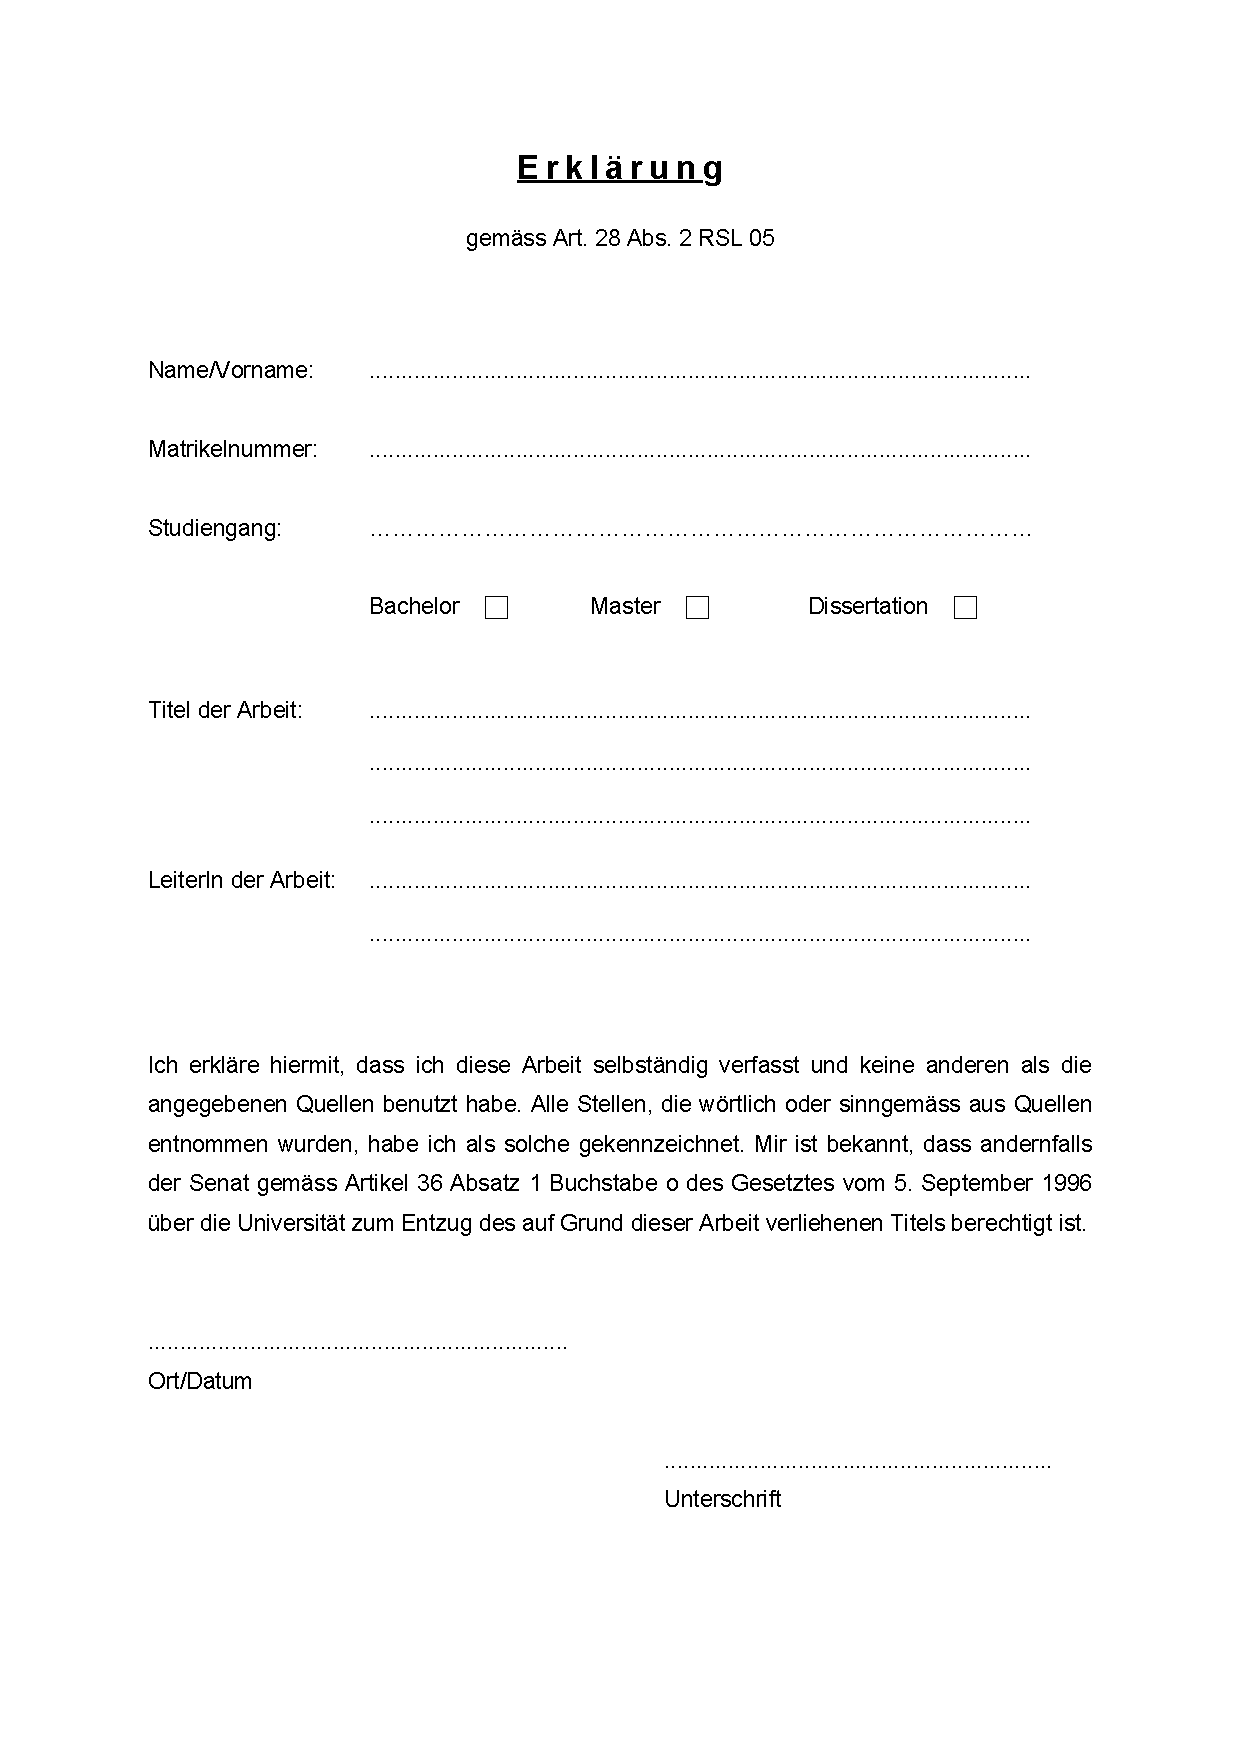
\includepdf{Erklaerung.pdf}

\end{document}
